\appendix
\section{Lab Report Policy}
\begin{enumerate}
\item Everyone needs to hand in their own lab report. If you work with someone
in the lab, then put that person's name on the lab report as a collaborator.
\item Each of you need to collect your own data and write your own report. I do
not want to see two reports with exactly the same data (even though everyone's
data will look similar) nor with the same lab report.
\end{enumerate}

\section{Typesetting with \LaTeX}
This document was created using the typesetting language \LaTeX, which allows
you to create very professional-looking documents with minimal effort. If you
are interested in learning how to create such documents using \LaTeX, I can
provide the code that generated this document as a template that you can start
with.

%%%%%%%%%%%%%%%%%%%%%%%%%%%%%%%%%%%%%%%%%%%%%%%%%%%%%%%%%%%%%%%%%%%%%%%%%%%%%
%%%%%%%%%%%%%%%%%%%%%%%%%%%%%%%%%%%%%%%%%%%%%%%%%%%%%%%%%%%%%%%%%%%%%%%%%%%%%


%%%%%%%%%%%%%%%%%%%%%%%%%%%%%%%%%%%%%%%%%%%%%%%%%%%%%%%%%%%%%%%%%%%%%%%%%%%%%

% Surround figure environment with turnpage environment for landscape presentation
\begin{turnpage}
\begin{figure*}[p]
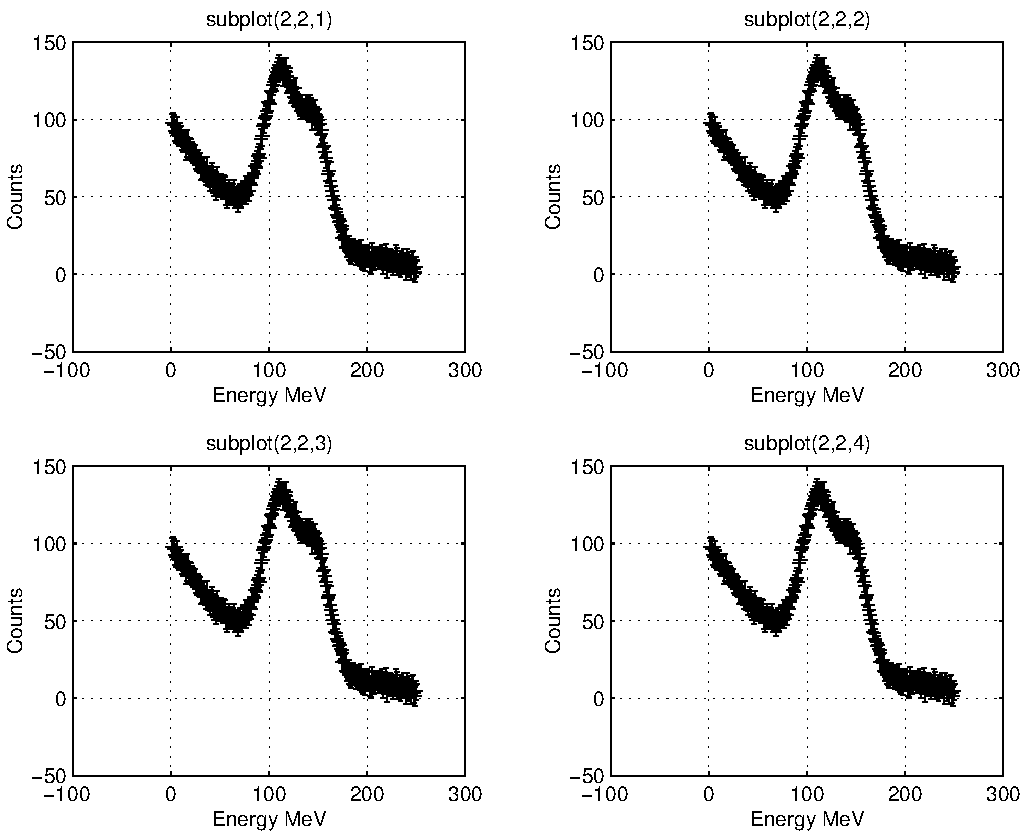
\includegraphics[width=20cm]{./figures/sample-fig5}
\caption{For very large plots where important detail might be lost
if too compressed. These full page graphics are usually best kept in
appendices so as not to impede the flow of the paper.  Note that
large tables can also be presented in this landscape environment if
desired.} 
\label{fig:landscapegraphic}
\end{figure*}
\end{turnpage}

% tables should appear as floats within the text
%
% Here is an example of the general form of a table:
% Fill in the caption in the braces of the \caption{} command. Put the label
% that you will use with \ref{} command in the braces of the \label{} command.
% Insert the column specifiers (l, r, c, d, etc.) in the empty braces of the
% \begin{tabular}{} command.
% The ruledtabular enviroment adds doubled rules to table and sets a
% reasonable default table settings.
% Use the table* environment to get a full-width table in two-column
% Add \usepackage{longtable} and the longtable (or longtable*}
% environment for nicely formatted long tables. Or use the the [H]
% placement option to break a long table (with less control than
% in longtable).
% \begin{table}%[H] add [H] placement to break table across pages
% \caption{\label{}}
% \begin{ruledtabular}
% \begin{tabular}{}
% Lines of table here ending with \\
% \end{tabular}
% \end{ruledtabular}
% \end{table}

% To convert program (e.g., C++ Fortran, Matlab, LaTeX\) listings to a
% form easily includable in a \LaTeX\ document
%
% type lgrind -s to see options
% lgrind -llatex -i sample-paper.tex > sampleinputtex
% creates a file sampleinput.tex which can then be included into this
% document simply by uncommenting the next line
%\lgrindfile{testinput.tex}

